\documentclass{beamer}

% german content
\usepackage[ngerman]{babel}

% bibliography
\usepackage[
backend=biber,
style=authoryear,
citestyle=authoryear,
autocite=footnote
]{biblatex}
\addbibresource{bibliography.bib}

% images
\usepackage{graphicx}
\graphicspath{ {images/} }

\title{Import/Export von saisonalen Produkten}
% \subtitle{}
\author[Dao, Gabele, Neidel, Neuthor, Spannbauer, Wiegandt]{
  Dao, Duc Trung \and\\
  Gabele, Jörg \and\\
  Neidel, Jonathan \and\\
  Neuthor, Marco \and\\
  Spannbauer, Daniel \and\\
  Wiegandt, Lisa-Marlen
}
\date{Januar 2020}
\institute{HTW Berlin, Angewandte Informatik}
\logo{
\includegraphics[width=1cm]{logo.png}}

% theme + color theme
\usetheme{Szeged}
\usecolortheme{whale}
% see: https://deic-web.uab.cat/~iblanes/beamer_gallery/index.html
\setbeamerfont{caption}{size=\Tiny}

\begin{document}
\frame{\titlepage}

\begin{frame}
\frametitle{Abstract}
Abstract here
\end{frame}

% show all section names
\begin{frame}
\frametitle{Table of Contents}
\tableofcontents
\end{frame}
% how to exclude a section from toc: https://tex.stackexchange.com/a/66633

\section{Theorie Import/Export}

\begin{frame}
\frametitle{Saisionale Produkte}
  \begin{itemize}
    \item Saisonale Produkte, wie Obst und Gemüse, stammen
      aus der Region und reifen zu bestimmten Zeiten im Jahr.
    \item  Verbesserte Lagerhaltungen machen viele Obst und
      Gemüsesorten länger haltbar.
    \item  Ein großer Vorteil von Saisonalen Produkten: Sie
      stammen aus der Region und erweisen einen kurzen
      Transportweg bis zum Verbraucher.
  \end{itemize}
\end{frame}


\begin{frame}
\frametitle{Export}
  \begin{itemize}
    \item
Unter Export versteht man den Transfer von Gütern und Dienstleistungen über
die Staatsgrenze eines Landes.
    \item
Deutschland wird oft als „Exportweltmeister“ bezeichnet.
    \item
Anhand des Warenwertes, ist China der größte Exporteur der Welt.
Was bedeutet Import?
    \item
Beim Import werden Waren, Güter und Dienstleistungen aus dem Ausland ins
  \end{itemize}
\end{frame}

\begin{frame}
\frametitle{Import}
  \begin{itemize}
    \item Beim Import werden Waren, Güter und Dienstleistungen aus dem Ausland ins
      Inland geliefert.
    \item Der Europäische Binnenmarkt und die Europäische Zollunion stellen einen
      einheitlichen Handelsraum dar.
    \item Hersteller aus der Europäischen Union profitieren davon enorm. Hingegen sind
      viele Einfuhren aus Ländern außerhalb der EU, mit Zöllen belegt.
  \end{itemize}
\end{frame}

\begin{frame}
\frametitle{Knappheit}
  \begin{itemize}
    \item
  Knappheit liegt vor, wenn die Nachfrage größer ist als
  das Angebot.
    \item
      \textbf{Zufällige Knappheit}: Unvorhersehbare Schwankungen
  im Angebot von Obst oder Gemüse.
      \begin{itemize}
        \item
  Hervorgerufen durch schlechte Ernten wegen Dürre oder
  Unwetter.
\item
Knappe Güter können zu erheblichen Preissteigerungen führen.
  \end{itemize}
      \end{itemize}
\end{frame}

\begin{frame}
\frametitle{Angebot}
  \begin{itemize}
    \item
Angebot bezeichnet die Menge eines Gutes, die die
Hersteller zu einem bestimmten Preis produzieren
können.
      \begin{itemize}
        \item
  Das Angebot abhängig von (Produktionsfaktoren, dem Stand
  der Produktionstechnik und den Erwartungen an den Markt).
      \end{itemize}
  \end{itemize}
\end{frame}

\begin{frame}
\frametitle{Nachfrage}
  \begin{itemize}
    \item
Nachfrage ist die Menge an Gütern, die die
Konsumenten zu einem bestimmten Preis kaufen wollen.

      \begin{itemize}
        \item
Hauptkriterien für den Kauf: Menge des Gutes, die Höhe des
eigenen Einkommens, persönlicher Geschmack, der Preis von
Substitutionsgütern und komplementären Gütern.
      \end{itemize}
  \end{itemize}
\end{frame}

\begin{frame}
\frametitle{Marktgleichgewicht}
  \begin{figure}[h]
    \centering
    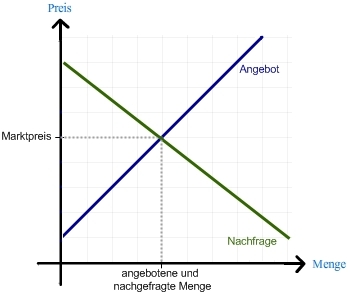
\includegraphics[height=6cm]{marktgleichgewicht}
    \caption{https://www.wiwiweb.de/mikrooekonomik/grundlagen/statik/gleichgewich.html}
  \end{figure}
\end{frame}
\begin{frame}
\frametitle{steigendes Angebot}
  \begin{figure}[h]
    \centering
    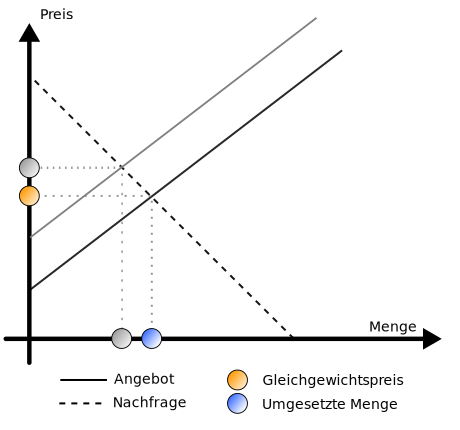
\includegraphics[height=6cm]{steigendes_angebot}
    \caption{https://de.wikipedia.org/wiki/Marktgleichgewicht}
  \end{figure}
\end{frame}
\begin{frame}
\frametitle{Economies of scale}

\begin{columns}
    \begin{column}{0.5\textwidth}
  \begin{figure}[h]
    \centering
      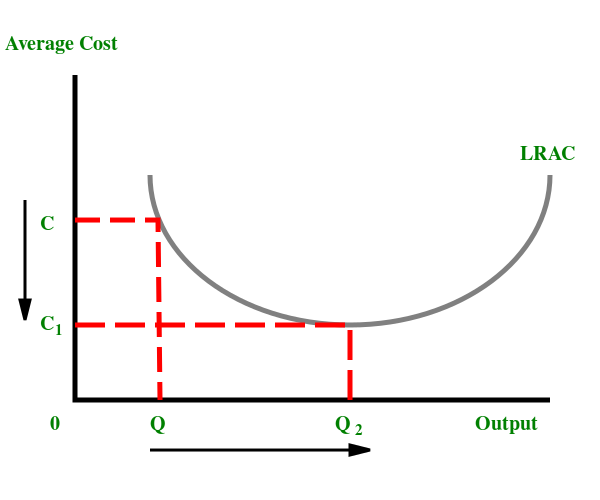
\includegraphics[width=0.9\textwidth]{economies_of_scale}
      \caption{https://napkinfinance.com/wp-content/uploads/2016/11/Economies-of-Scale-final.jpg}
  \end{figure}
    \end{column}
    \begin{column}{0.5\textwidth}
    \begin{itemize}
    \item
  Mit Ausweitung der zu
  erwirtschaftenden Gütern,
  wird eine größere Menge
  dieser, auf die
  gleichbleibenden Fixkosten
  aufgeteilt.
\item
  Somit sind die Fixkosten pro
  Stück geringer.

    \end{itemize}
    \end{column}
\end{columns}
\end{frame}

% \begin{frame}
% \frametitle{<++>}
% <++>
% \end{frame}

% bibliography
% \break
% \printbibliography

\end{document}
